\section{Results}
\subsection{Measurements for spring constant}
    From the raw spring length measurement data in Table \ref{spring}, we obtain the change amount of the spring length by $\Delta L_i=L_i-L_0$ in Table \ref{spring*}.

    Since the acceleration due to gravity is exactly $9.794m/s^2$, we obtain the weights of weight stacks from their masses, as shown in Table \ref{weight}.
    \begin{table}[h]
        \centering
        \begin{tabular}{|c|c|c|c|c|c|}
            \hline
            \multicolumn{6}{|c|}{Unit: $[\times 10^{-2}m]\pm 0.01[\times 10^{-2}m]$}\\ \hline
            No. & spring 1 & No. & spring 2 & No. & series\\ \hline
            $L_0$ & 2.25 & $L_0$ & 2.84 & $L_0$ & 5.06\\ \hline
            $L_1$ & 4.40 & $L_1$ & 4.96	& $L_1$ & 9.25\\ \hline
            $L_2$ & 6.56 & $L_2$ & 7.08 & $L_2$ & 13.38\\ \hline
            $L_3$ & 8.70 & $L_3$ & 9.18	& $L_3$ & 17.60\\ \hline
            $L_4$ & 10.78 & $L_4$ & 11.25 & $L_4$ & 21.98\\ \hline
            $L_5$ & 12.85 & $L_5$ & 13.30 & $L_5$ & 26.09\\ \hline
            $L_6$ & 15.03 & $L_6$ &	15.42 & $L_6$ &	30.31\\ \hline
        \end{tabular}
        \caption{Spring constant measurement data}\label{spring}
    \end{table}
    \begin{table}[htbp]
        \centering
        \begin{tabular}{|c|c|c|c|c|c|}
            \hline
            \multicolumn{6}{|c|}{Unit: $[\times 10^{-2}m]\pm 0.01[\times 10^{-2}m]$}\\ \hline
            No. & spring 1 & No. & spring 2 & No. & series\\ \hline
            $\Delta {L_1}$ & 2.15 & $\Delta {L_1}$ & 2.12 & $\Delta {L_1}$ & 4.19\\ \hline
            $\Delta {L_2}$ & 4.31 & $\Delta {L_2}$ & 4.24 & $\Delta {L_2}$ & 8.32\\ \hline
            $\Delta {L_3}$ & 6.45 & $\Delta {L_3}$ & 6.34 & $\Delta {L_3}$ & 12.54\\ \hline
            $\Delta {L_4}$ & 8.53 & $\Delta {L_4}$ & 8.41 & $\Delta {L_4}$ & 16.92\\ \hline
            $\Delta {L_5}$ & 10.60 & $\Delta {L_5}$ & 10.46 & $\Delta {L_5}$ & 21.03\\ \hline
            $\Delta {L_6}$ & 12.78 & $\Delta {L_6}$ & 12.58 & $\Delta {L_6}$ & 25.25\\ \hline
        \end{tabular}
        \caption{Calculated spring measurement data}\label{spring*}
    \end{table}
    \begin{table}[htbp]
        \centering
        \begin{tabular}{|c|c|c|}
            \hline
            & $m[\times 10^{-3}kg]\pm 0.01[\times 10^{-3}kg]$ & $W[\times 10^{-3}N]\pm 0.1[\times 10^{-3}N]$\\ \hline
            1 & 4.83 & 47.3\\ \hline
            2 & 9.65 & 94.5\\ \hline
            3 & 14.50 & 142.0\\ \hline
            4 & 19.24 & 188.4\\ \hline
            5 & 23.99 & 235.0\\ \hline
            6 & 28.80 & 282.1\\ \hline            
        \end{tabular}
        \caption{Weight measurement data}\label{weight}
    \end{table}
    The relation between the elastic force and the change of spring length is linear.Using the least-squares method, we can calculate the most optimal estimate of the slope and intercept. The errorbars of $W$ and $\Delta_L$ are based on their own combined uncertainties, which is just their type $B$ uncertainties $\Delta_B$ in this case. Specific error calculaton is included in section 5.

    The errorbar is \textbf{not clear enough} because the error is relatively \textbf{small}. The sample calculation of $k_1$ done by Matlab is also shown here. The fitting curve in Figure \ref{k_1} is based on Table \ref{k1data}.
    \begin{table}
        \centering
        \begin{tabular}{|c|c|c|c|c|}
            \hline
            No. & $\Delta_L[m]$ & $u_{\Delta_L}[m]$ & $W[N]$ & $u_{W}[N]$\\ \hline
            1 & 0.0215 & 0.00014 & 0.04730 & 0.0001\\ \hline
            1 & 0.0431 & 0.00014& 0.09451 & 0.0001\\ \hline
            1 & 0.0645 & 0.00014& 0.1420 & 0.0001\\ \hline
            1 & 0.0853 & 0.00014& 0.1884 & 0.0001\\ \hline
            1 & 0.1060 & 0.00014& 0.2350 & 0.0001\\ \hline
            1 & 0.1278 & 0.00014& 0.2821 & 0.0001\\ \hline
        \end{tabular}
        \caption{Data for $W vs. \Delta L$ of spring 1 in Figure \ref{k_1}}\label{k1data}
    \end{table}
    \begin{figure}[h]    
        \begin{minipage}{0.5\linewidth}
            \[
            \begin{split}
                k_1&=\frac{\overline{\Delta LW}-\overline{\Delta L}\cdot\overline{W}}{\overline{\Delta L^2}-\overline{\Delta L}^2}\\[0.2cm]
                &\approx \frac{1.52\times10^{-2}-7.47\times10^{-2}\times0.165}{68.9\times10^{-4}-55.8\times10^{-4}}\\[0.2cm]
                &=2.22\pm 0.02kg/s^2.\\[0.4cm]
                u_{r,k_1}&=0.9\%
                %b_1&=\overline{W}-k_1\overline{\Delta_L}\\[0.2cm]
                %&\approx 0.1649\times 2.22 \times 0.07470\\[0.2cm]
                %&=(-6.25\pm 12.5)\times10^{-4}N.
            \end{split}
            \]
        \end{minipage}
        \begin{minipage}{0.4\linewidth}
            \centering
            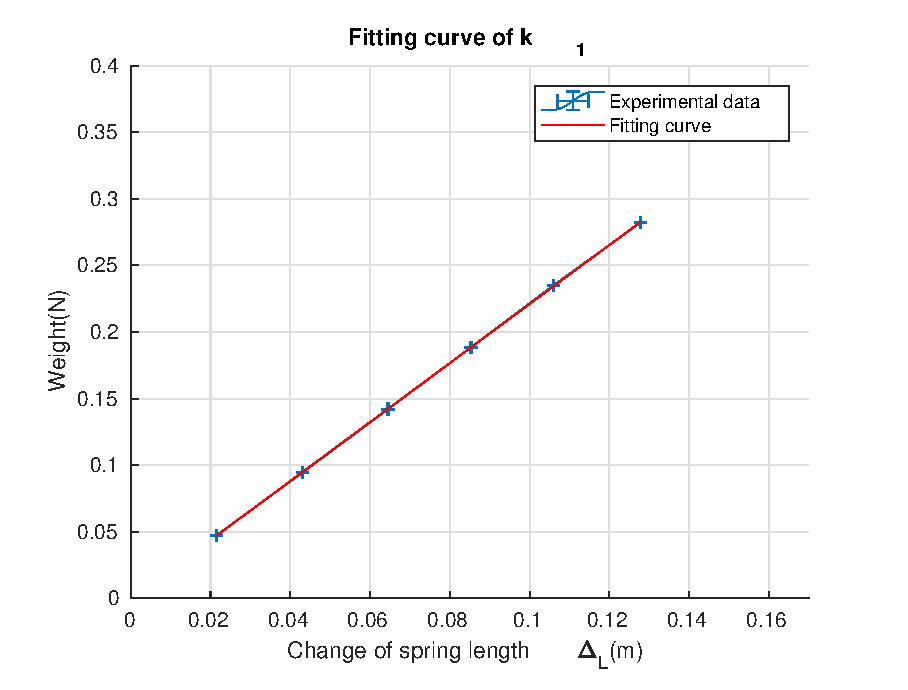
\includegraphics[height=6.7cm]{images/k1.eps}
            \caption{Fitting curve of spring 1}\label{k_1}
        \end{minipage}
    \end{figure}
    \newpage
    \begin{figure}[!h]
        \centering
        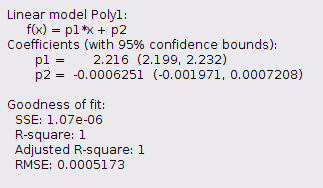
\includegraphics[height=5.8cm]{images/k1info.png}
        \caption{Information of fit in Figure \ref{k_1}}\label{k1info}
    \end{figure}
    Simliarly, we obtain $k_2$ and $k_3$.
    \begin{table}[!htbp] \small
        \centering
        \begin{tabular}{|c|c|c|c|c|}
            \hline
            No. & $\Delta_L[m]$ & $u_{\Delta_L}[m]$ & $W[N]$ & $u_{W}[N]$\\ \hline
            1 & 0.0212 & 0.00014& 0.04730 & 0.0001\\ \hline
            1 & 0.0424 & 0.00014& 0.09451 & 0.0001\\ \hline
            1 & 0.0634 & 0.00014& 0.1420 & 0.0001\\ \hline
            1 & 0.0841 & 0.00014& 0.1884 & 0.0001\\ \hline
            1 & 0.1046 & 0.00014& 0.2350 & 0.0001\\ \hline
            1 & 0.1258 & 0.00014& 0.2821 & 0.0001\\ \hline
        \end{tabular}
        \caption{Data for $W vs. \Delta_L$ of spring 2 in Figure \ref{k_2}}\label{k2data}
    \end{table}
    \begin{figure}[!h]
        \centering
        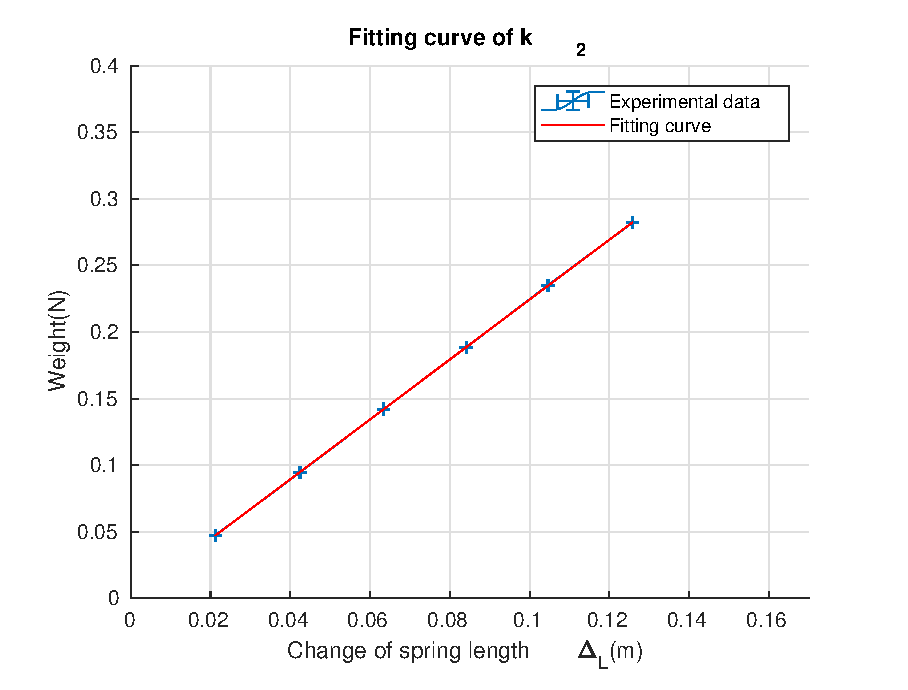
\includegraphics[height=6cm]{images/k2.eps}
        \caption{Fitting curve of spring 2}\label{k_2}
    \end{figure}
    \begin{figure}[!h]
        \centering
        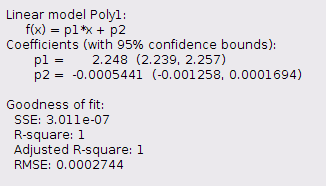
\includegraphics[height=5cm]{images/k2info.png}
        \caption{Information of fit in Figure \ref{k_2}}\label{k2info}
    \end{figure}
    \[
        k_2\approx 2.25\pm 0.010kg/s^2, \quad u_{r,k_2}=0.4\%
        %b_2&\approx (-5.44\pm 70) \times10^{-4}N.
    \]
    \begin{table}[!ht] \small
        \centering
        \begin{tabular}{|c|c|c|c|c|}
            \hline
            No. & $\Delta_L[m]$ & $u_{\Delta_L}[m]$ & $W[N]$ & $u_{W}[N]$\\ \hline
            1 & 0.0419 & 0.00014& 0.04730 & 0.0001\\ \hline
            2 & 0.0832 & 0.00014& 0.09451 & 0.0001\\ \hline
            3 & 0.1254 & 0.00014& 0.1420 & 0.0001\\ \hline
            4 & 0.1692 & 0.00014& 0.1884 & 0.0001\\ \hline
            5 & 0.2103 & 0.00014& 0.2350 & 0.0001\\ \hline
            6 & 0.2525 & 0.00014& 0.2821 & 0.0001\\ \hline
        \end{tabular}
        \caption{Data for $W vs. \Delta_L$ of spring series in Figure \ref{k_3}}\label{k3data}
    \end{table}
    \newpage
    \begin{figure}[h]
        \centering    
        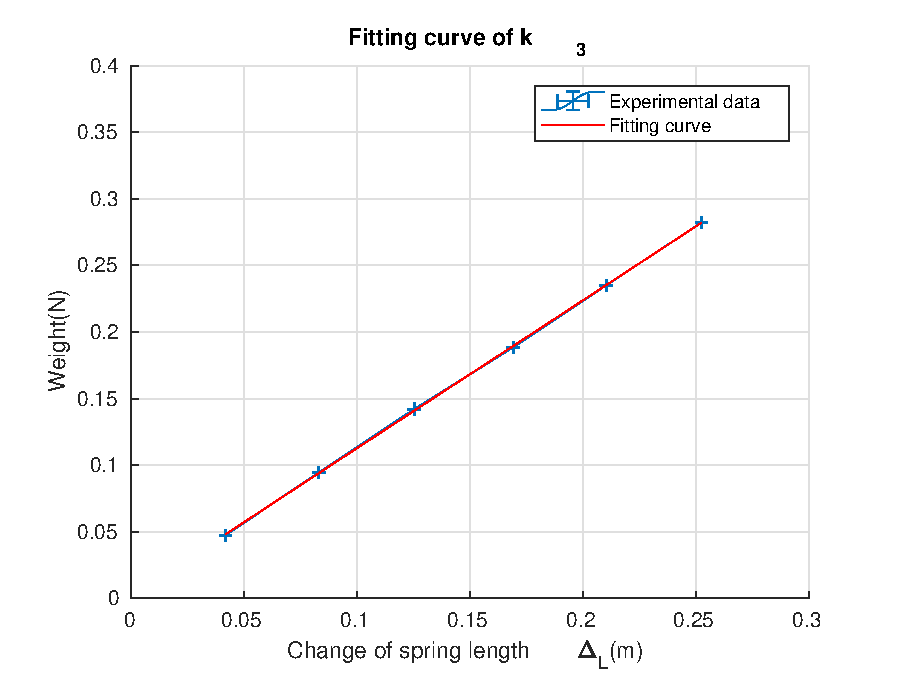
\includegraphics[height=7cm]{images/k3.eps}
        \caption{Fitting curve of series of spring 1 and spring 2}\label{k_3}
    \end{figure}
    \begin{figure}[!h]
        \centering
        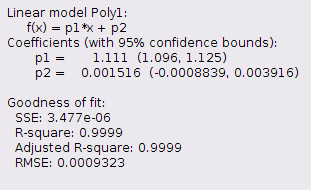
\includegraphics[height=5cm]{images/k3info.png}
        \caption{Information of fit in Figure \ref{k_3}}\label{k3info}
    \end{figure}
    \[
        k_3\approx 1.11\pm 0.017kg/s^2, \quad u_{r,k_3}=1.5\%
        %b_3&\approx (15.1\pm 20)\times10^{-4}N.
    \]

    However, $k_3$ could be theoretically calculated by $k_1$ and $k_2$. This will be further discussed in section 5.\\

\subsection{Relation between the period $T$ and the mass $M$}
    In this experiment we use I-shape shutter to block the photoelectric gate. The mass data are listed in Table \ref{M} and. The effective mass in Table \ref{M} is the sum of $m_{objI}$ and the mass of weights in Table \ref{weight}.

    \begin{table}[h]
        \centering
        \begin{tabular}{|c|c|}
            \hline
            object with I-shape & $m_{objI}=176.55\pm 0.01[\times10^{-3}kg]$\\ \hline
            object with U-shape & $m_{objU}=186.75\pm 0.01[\times10^{-3}kg]$\\ \hline
            mass of spring 1 & $m_{spr1}=10.74\pm 0.01[\times10^{-3}kg]$\\ \hline
            mass of spring 2 & $m_{spr2}=10.77\pm 0.01[\times10^{-3}kg]$\\ \hline
            equivalent mass & $M_I=m_{objI}+\frac{1}{3}m_{spr1}+\frac{1}{3}m_{spr2}=183.72\pm 0.015[\times10^{-3}kg]$\\ \hline
            equivalent mass & $M_U=m_{objU}+\frac{1}{3}m_{spr1}+\frac{1}{3}m_{spr2}=193.92\pm 0.015[\times10^{-3}kg]$\\ \hline
        \end{tabular}
        \caption{Mass measurement data}\label{M}
    \end{table}
    \vspace{1cm}
    %\begin{table}[h]
    %    \centering
    %    \begin{tabular}{|c|c|c|c|c|c|c|}
    %        \hline
    %        \multicolumn{6}{|c|}{Ten periods $[\times10^{-3}s]\pm0.1[\times10^{-3}s]$} & Effective mass\\ \hline
    %        \multicolumn{2}{|c|}{horizontal} & \multicolumn{2}{|c|}{incline 1} & \multicolumn{2}{|c|}{incline 2} & $[\times10^{-3}]\pm 0.01[\times10^{-3}kg]$\\ \hline
    %        $m_1$ & 12798.9 & $m_1$ & 12804.1 & $m_1$ & 12800.1 & 188.55\\ \hline
    %        $m_1$ & 12964.9 & $m_2$ & 12957.0 & $m_2$ & 12955.4 & 193.37\\ \hline
    %        $m_1$ & 13127.2 & $m_3$ & 13123.7 & $m_3$ & 13127.0 & 198.22\\ \hline
    %        $m_1$ & 13282.6 & $m_4$ & 13282.7 & $m_4$ & 13275.6 & 202.96\\ \hline
    %        $m_1$ & 13436.3 & $m_5$ & 13439.3 & $m_5$ & 13436.3 & 207.71\\ \hline
    %        $m_1$ & 13592.4 & $m_6$ & 13591.6 & $m_6$ & 13594.9 & 212.52\\ \hline
    %    \end{tabular}
    %    \caption{Measurement data for the T vs. M relation}\label{T}
    %\end{table}
    Again using the least-squares method we can plot the fitting curve of $T^2 vs. M$ (see Figure \ref{tm}). The errorbar is still \textbf{not clear} though.

    \begin{table}[h] \small
        \centering
        \begin{tabular}{|c|c|c|c|c|}
            \hline
            No. & $M[kg]$ & $u_{M}[kg]$ & $T^2[s^2]$ & $u_{T^2}[s^2]$\\ \hline
            1 & 0.18855 & 0.000015 & 1.63812 & 0.00003\\ \hline
            2 & 0.19337 & 0.000015 & 1.68089 & 0.00003\\ \hline
            3 & 0.19822 & 0.000015 & 1.72323 & 0.00003\\ \hline
            4 & 0.20296 & 0.000015 & 1.76427 & 0.00003\\ \hline
            5 & 0.20771 & 0.000015 & 1.80534 & 0.00003\\ \hline
            6 & 0.21252 & 0.000015 & 1.84753 & 0.00003\\ \hline
        \end{tabular}
        \caption{Data for $T^2 vs. M$ for the horizontal track in Figure \ref{tm}}\label{tmdata}
    \end{table}
    \begin{figure}[!h]
        \centering    
        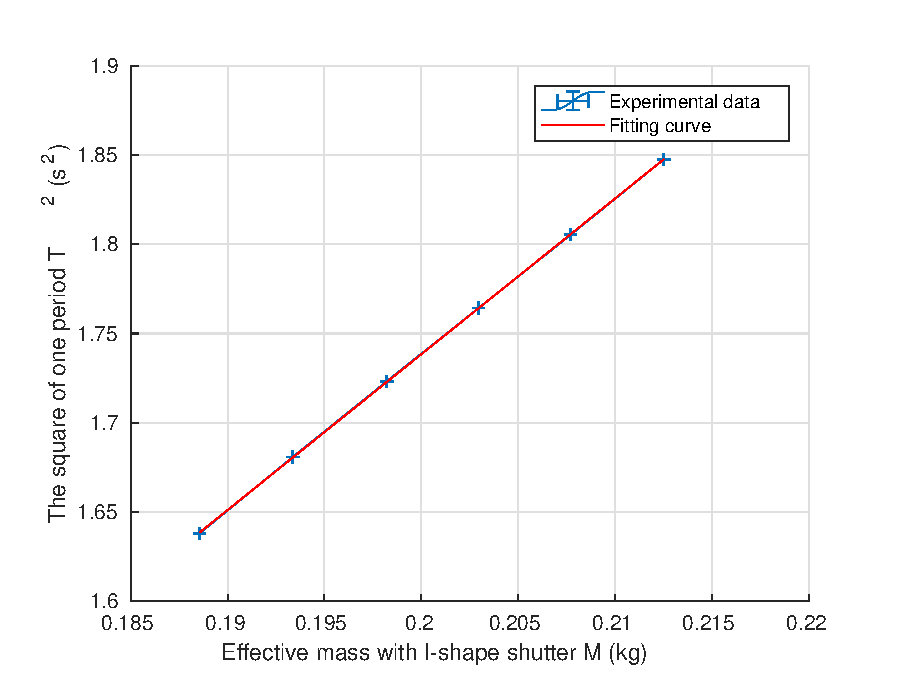
\includegraphics[height=9cm]{images/tm.eps}     
        \caption{$T^2 vs. M$ for the horizontal track.$\quad slope_{hor}=8.72\pm 0.05s^2/kg,\quad u_{r,hor}=0.6\%.$}\label{tm}
    \end{figure}
    \begin{figure}[!h]
        \centering
        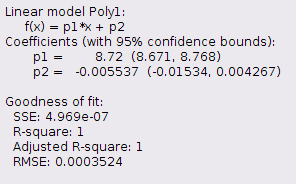
\includegraphics[height=5cm]{images/tminfo.png}
        \caption{Information of fit in Figure \ref{tm}}\label{tminfo}
    \end{figure}
    \begin{table}
        \centering
        \begin{tabular}{|c|c|c|c|c|}
            \hline
            No. & $M[kg]$ & $u_{M}[kg]$ & $T^2[s^2]$ & $u_{T^2}[s^2]$\\ \hline
            1 & 0.18855 & 0.000015 & 1.63945 & 0.00003\\ \hline
            2 & 0.19337 & 0.000015 & 1.67884 & 0.00003\\ \hline
            3 & 0.19822 & 0.000015 & 1.72232 & 0.00003\\ \hline
            4 & 0.20296 & 0.000015 & 1.76430 & 0.00003\\ \hline
            5 & 0.20771 & 0.000015 & 1.80615 & 0.00003\\ \hline
            6 & 0.21252 & 0.000015 & 1.84732 & 0.00003\\ \hline
        \end{tabular}
        \caption{Data for $T^2 vs. M$ for incline 1 in Figure \ref{tmi1}}\label{tmi1data}
    \end{table}
    \begin{figure}[!h]
        \centering
        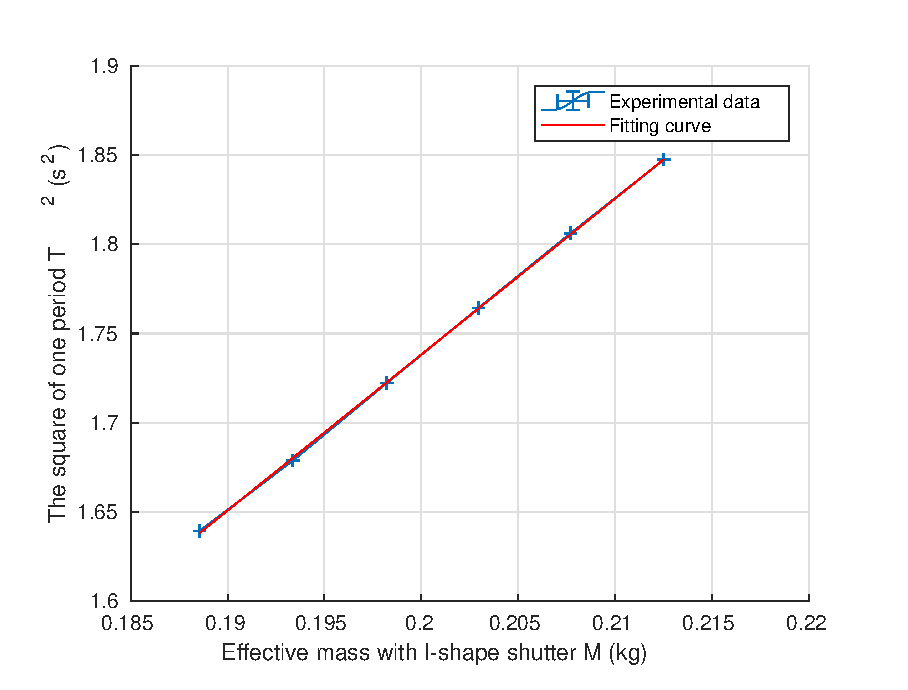
\includegraphics[height=6cm]{images/tmi1.eps}
        \caption{$T^2 vs. M$ for incline 1. $\quad slope_{inc1}=8.73\pm 0.14s^2/kg,\quad u_{r,inc1}=1.6\%.$}\label{tmi1}
    \end{figure}
    \begin{figure}[!h]
        \centering
        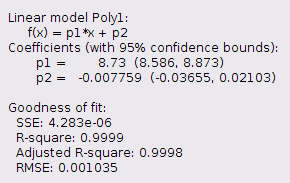
\includegraphics[height=5cm]{images/tmi1info.png}
        \caption{Information of fit in Figure \ref{tmi1}}\label{tmi1info}
    \end{figure}
    \begin{table}\small
        \centering
        \begin{tabular}{|c|c|c|c|c|}
            \hline
            No. & $M[kg]$ & $u_{M}[kg]$ & $T^2[s^2]$ & $u_{T^2}[s^2]$\\ \hline
            1 & 0.18855 & 0.000015 & 1.63843 & 0.00003\\ \hline
            2 & 0.19337 & 0.000015 & 1.67842 & 0.00003\\ \hline
            3 & 0.19822 & 0.000015 & 1.72318 & 0.00003\\ \hline
            4 & 0.20296 & 0.000015 & 1.76242 & 0.00003\\ \hline
            5 & 0.20771 & 0.000015 & 1.80534 & 0.00003\\ \hline
            6 & 0.21252 & 0.000015 & 1.84821 & 0.00003\\ \hline
        \end{tabular}
        \caption{Data for $T^2 vs. M$ for incline 2 in Figure \ref{tmi2}}\label{tmi2data}
    \end{table}

    \begin{figure}[!h]
        \centering
        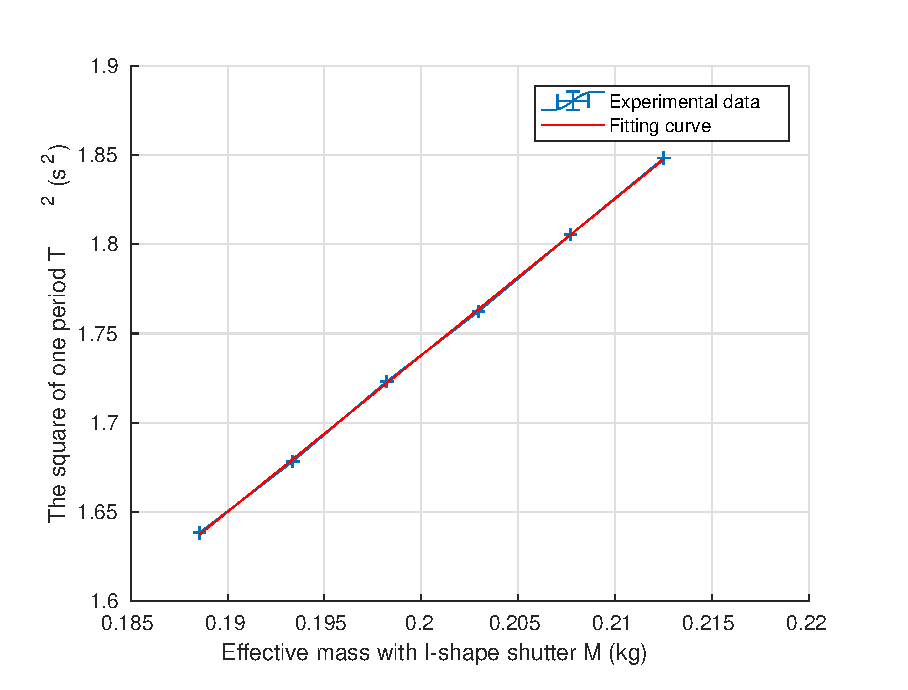
\includegraphics[height=8cm]{images/tmi2.eps}
        \caption{$T^2 vs. M$ for incline 2. $\quad slope_{inc2}=8.76\pm 0.17s^2/kg,\quad u_{r,inc2}=1.9\%.$}\label{tmi2}
    \end{figure}
    \begin{figure}[h]
        \centering
        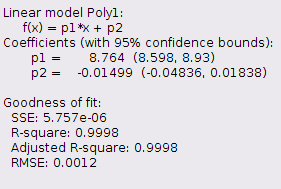
\includegraphics[height=5cm]{images/tmi2info.png}
        \caption{Information of fit in Figure \ref{tmi2}}\label{tmi2info}
    \end{figure}
    From the results above, we can conclude that therelation between $T^2$ and $M$ is that $T^2\propto M$. Whether it's incline or horizontal will \textbf{not} affect the relation. 

\subsection{Relation between period $T$ and amplitude $A$}
    \begin{table}[h] \small
        \centering
        \begin{tabular}{|c|c|c|c|c|}
            \hline
            No. & $A[m]$ & $u_{A}[m]$ & $T[s]$ & $u_{T}[s]$\\ \hline
            1 & 0.05 & 0.001 & 1.26451 & 0.0001\\ \hline
            2 & 0.10 & 0.001 & 1.26361 & 0.0001\\ \hline
            3 & 0.15 & 0.001 & 1.26287 & 0.0001\\ \hline
            4 & 0.20 & 0.001 & 1.26358 & 0.0001\\ \hline
            5 & 0.25 & 0.001 & 1.26362 & 0.0001\\ \hline
            6 & 0.30 & 0.001 & 1.26360 & 0.0001\\ \hline
        \end{tabular}
        \caption{Data for $A\ vs.\ T$ in Figure \ref{at}}\label{atdata}
    \end{table}
    \begin{figure}[!h]
        \centering
        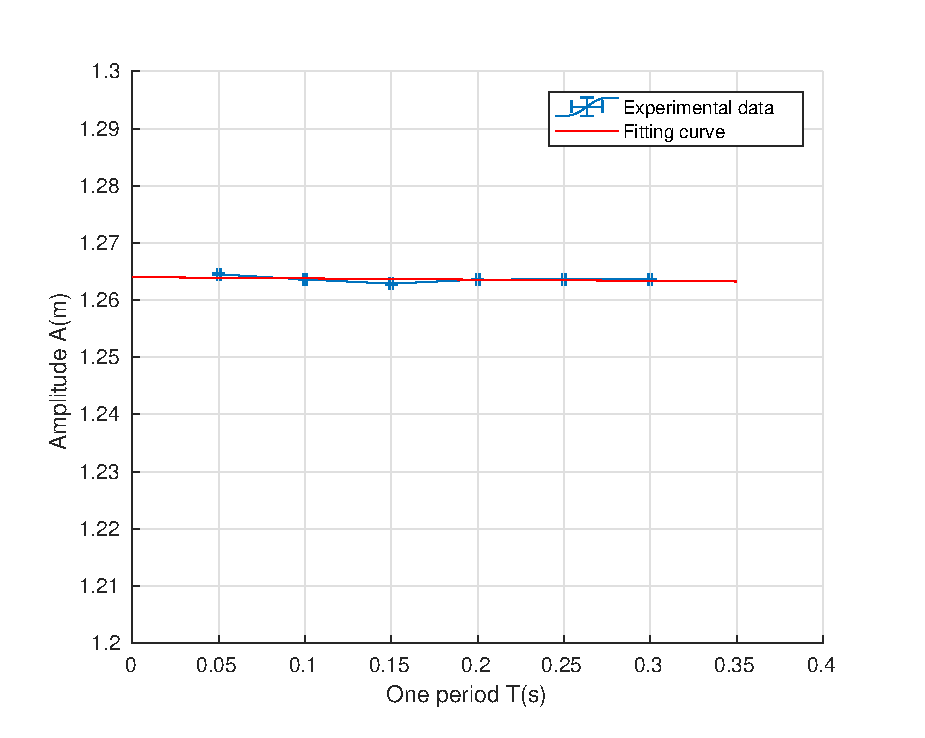
\includegraphics[height=7cm]{images/at.eps}
        \caption{Fitting curve of $T\ vs.\ A$, $\quad slope=(-2.18\pm7)\times10^{-3}s/m, \quad u_r=300\%$}\label{at}
    \end{figure}
    \vspace{0.6cm}
    \begin{figure}[h]
        \centering
        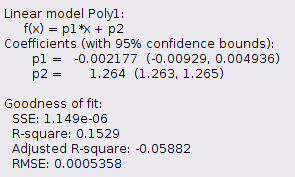
\includegraphics[height=5cm]{images/atinfo.png}
        \caption{Information of fit in Figure \ref{at}}\label{atinfo}
    \end{figure}
    To figure out whether $T$ depends on A, we need to calculate the correlation coefficient $\gamma$. The result generated by Matlab shows that
    \[
        \gamma_{A,T}=\frac{cov(A,T)}{s_A\cdot s_T}=\frac{\sum(A-\bar{A})(T-\bar{T})}{ns_A\cdot s_T}\approx -0.391.
    \]
    In fact we know that the period $T$ does not depend on $A$, which means the theoretical value of $\gamma$ should be $0$. Nevertheless, the experimental value shows that $T$ and $A$ is weakly correlated. This will be discussed in section 6.

\subsection{Relation between the maximum speed and the amplitude}
    First, we need the average values of $x_{in}$ and $x_{out}$ using the data from Table \ref{x}.
    \begin{table}[h] \small
        \centering
        \begin{tabular}{|c|c|c|}
            \hline
            No. & $x_{in}[\times10^{-3}m]\pm 0.02[\times10^{-3}m]$ & $x_{out}[\times10^{-3}m]\pm 0.02[\times10^{-3}m]$\\ \hline
            1 & 4.48 & 15.40\\ \hline
            2 & 4.52 & 15.40\\ \hline
            3 & 4.46 & 15.42\\ \hline
        \end{tabular}
        \caption{Data for the calculation of $\Delta x$}\label{x}
    \end{table}
    \[
    \begin{split}
        x_{in}&=\frac{1}{3}\sum_{i=1}^{3}x_{in,i}=\frac{0.00448+0.00452+0.00446}{3}\\
        &=(4.49\pm0.08)\times10^{-3}m,\quad u_{r,x_{in}}=1.8\%.\\[0.4cm]
        x_{out}&=\frac{1}{3}\sum_{i=1}^{3}x_{out,i}=\frac{0.01540+0.01540+0.01542}{3}\\
        &=(15.41\pm0.03)\times10^{-3}m,\quad u_{r,x_{out}}=0.2\%.\\
    \end{split}
    \]
    \[
    \begin{split}
        \Delta x&=(x_{in}+x_{out})/2\\
        &=(9.95\pm0.04)\times10^{-3}m,\quad u_{r,\Delta x}=0.4\%.
    \end{split}
    \]

    \begin{table}[h] \small
        \centering
        \begin{tabular}{|c|c|c|c|c|}
            \hline
            No. & $A^2[m^2]$ & $u_{A^2}[m^2]$ & $v_{max}^2[m^2/s^2]$ & $u_{v_{max}^2}[m^2/s^2]$\\ \hline
            1 & 0.0025 & 0.0001 & 0.0570 & 0.0005\\ \hline
            2 & 0.0100 & 0.0002 & 0.233 & 0.002  \\ \hline
            3 & 0.0225 & 0.0003 & 0.518 & 0.004  \\ \hline
            4 & 0.0400 & 0.0004 & 0.907 & 0.007  \\ \hline
            5 & 0.0625 & 0.0005 & 1.41 & 0.012   \\ \hline
            6 & 0.0900 & 0.0006 & 2.00 & 0.017   \\ \hline
        \end{tabular}
        \caption{Data for the fitting curve in Figure \ref{va}}\label{vadata}
    \end{table}
    \begin{figure}[!h]
        \centering
        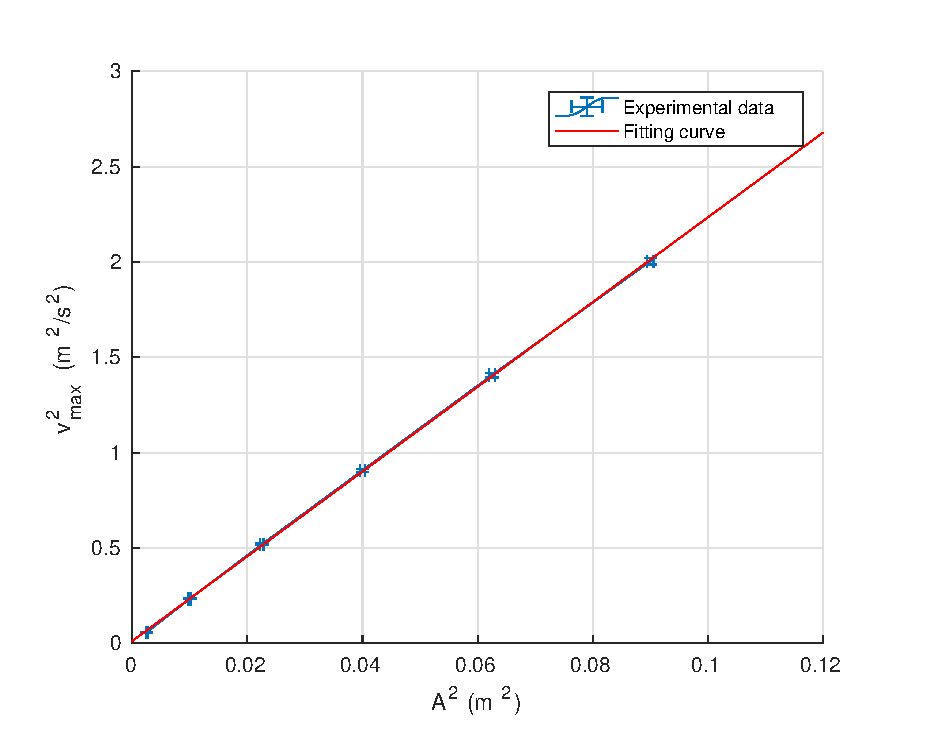
\includegraphics[height=6cm]{images/va.eps}
        \caption{Fitting curve of $v_{max}^2\ vs.\ A^2$, $\quad slope=22.22\pm0.31s^{-2}, \quad u_r=1.4\%$}\label{va}
    \end{figure}
    \begin{figure}[!h]
        \centering
        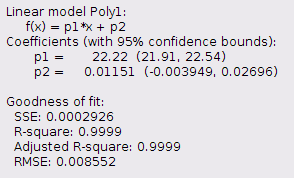
\includegraphics[height=5cm]{images/vainfo.png}
        \caption{Information of fit in Figure \ref{va}}\label{vainfo}
    \end{figure}